\documentclass[conference]{IEEEtran}
\usepackage{cite}
\usepackage{amsmath,amssymb,amsfonts}
\usepackage{graphicx}
\usepackage{textcomp}
\usepackage{xcolor}
\usepackage{url}
\usepackage{booktabs}

\begin{document}

\title{Task [B3]: [Predicting Star Ratings of E-Commerce Clothing Reviews]}

\author{\IEEEauthorblockN{Muhammad Zaryab Attiq}
\IEEEauthorblockA{Roll No. 70176119 \quad Section A\\
Repository: \url{https://github.com/Muhammad-Zaryab-Attiq/AI101-ML-Assignment-70176119}\\
Instructor: Dr. Muhammad Awais, AI Architect}
}

\maketitle

\section{Introduction}
Customer reviews in online apparel retail provide indispensable feedback for conversion optimization and inventory management. In this work, we address the challenge of predicting ordinal 1-to-5 star ratings from 22,641 women's e-commerce clothing reviews by combining unstructured customer text with structured administrative metadata (customer age, positive feedback count, review word count, and product departments). To preserve scientific validity, we enforce the leakage rule by omitting the concurrent \texttt{Recommended IND} feature. We perform a three-way ablation study (structured-only vs. text-only vs. multimodal), benchmark class balancing methods, and analyze a re-framed 3-class commercial sentiment framing (Negative, Neutral, Positive), which elevates accuracy from 61.35\% to 81.63\%.

\section{Problem Statement}
Given an input record $x = (x_{\text{text}}, x_{\text{num}}, x_{\text{cat}})$, the primary objective is to predict the discrete ordinal rating $y \in \{1, 2, 3, 4, 5\}$. Because the distribution exhibits severe positive skew (55.4\% are 5-star reviews), overall accuracy is misleading. Evaluation relies on Macro-Averaged F1-Score:
\begin{equation}
\text{Macro-F1} = \frac{1}{5} \sum_{c=1}^5 F_{1,c}
\end{equation}
and Ordinal Mean Absolute Error (MAE): $\frac{1}{N} \sum_{i=1}^N |y_i - \hat{y}_i|$, measuring average star displacement.

\section{Dataset Used}
We employ the Women's E-Commerce Clothing Reviews dataset from Kaggle~\cite{nicapotato2018}. The cleaned corpus contains 22,641 valid reviews. Features comprise the review narrative, customer age, positive feedback count, division, department, and apparel class.

\section{Leakage Rule & Dataset Statistics}
\textbf{Data Leakage Constraint:} The feature \texttt{Recommended IND} is strictly excluded. Because consumers tick the recommendation box concurrently with awarding star ratings, this feature is unavailable at inference time. Including it constitutes severe label leakage.
Table~\ref{tab:dataset_stats} displays the class breakdown: 5 stars (55.4\%), 4 stars (21.7\%), 3 stars (12.5\%), 2 stars (6.8\%), and 1 star (3.6\%). Dissatisfied reviewers write longer descriptions (median 68 words for 2-star vs. 52 words for 5-star).

\begin{table}[htbp]
\caption{Dataset statistics and star distribution.}
\label{tab:dataset_stats}
\centering
\begin{tabular}{lr}
\toprule
\textbf{Property} & \textbf{Value} \\
\midrule
Total clean reviews & 22,641 \\
Target scale & Discrete Ordinal [1--5 stars] \\
Class skew (5-star majority) & 12,540 samples (55.39\%) \\
Minority class (1-star) & 821 samples (3.63\%) \\
Excluded leakage feature & \texttt{Recommended IND} \\
Train / validation / test split & 15,848 / 3,396 / 3,397 (70/15/15) \\
Preprocessing & ColumnTransformer (TF-IDF + OneHot) \\
\bottomrule
\end{tabular}
\end{table}

\begin{figure}[htbp]
\centering
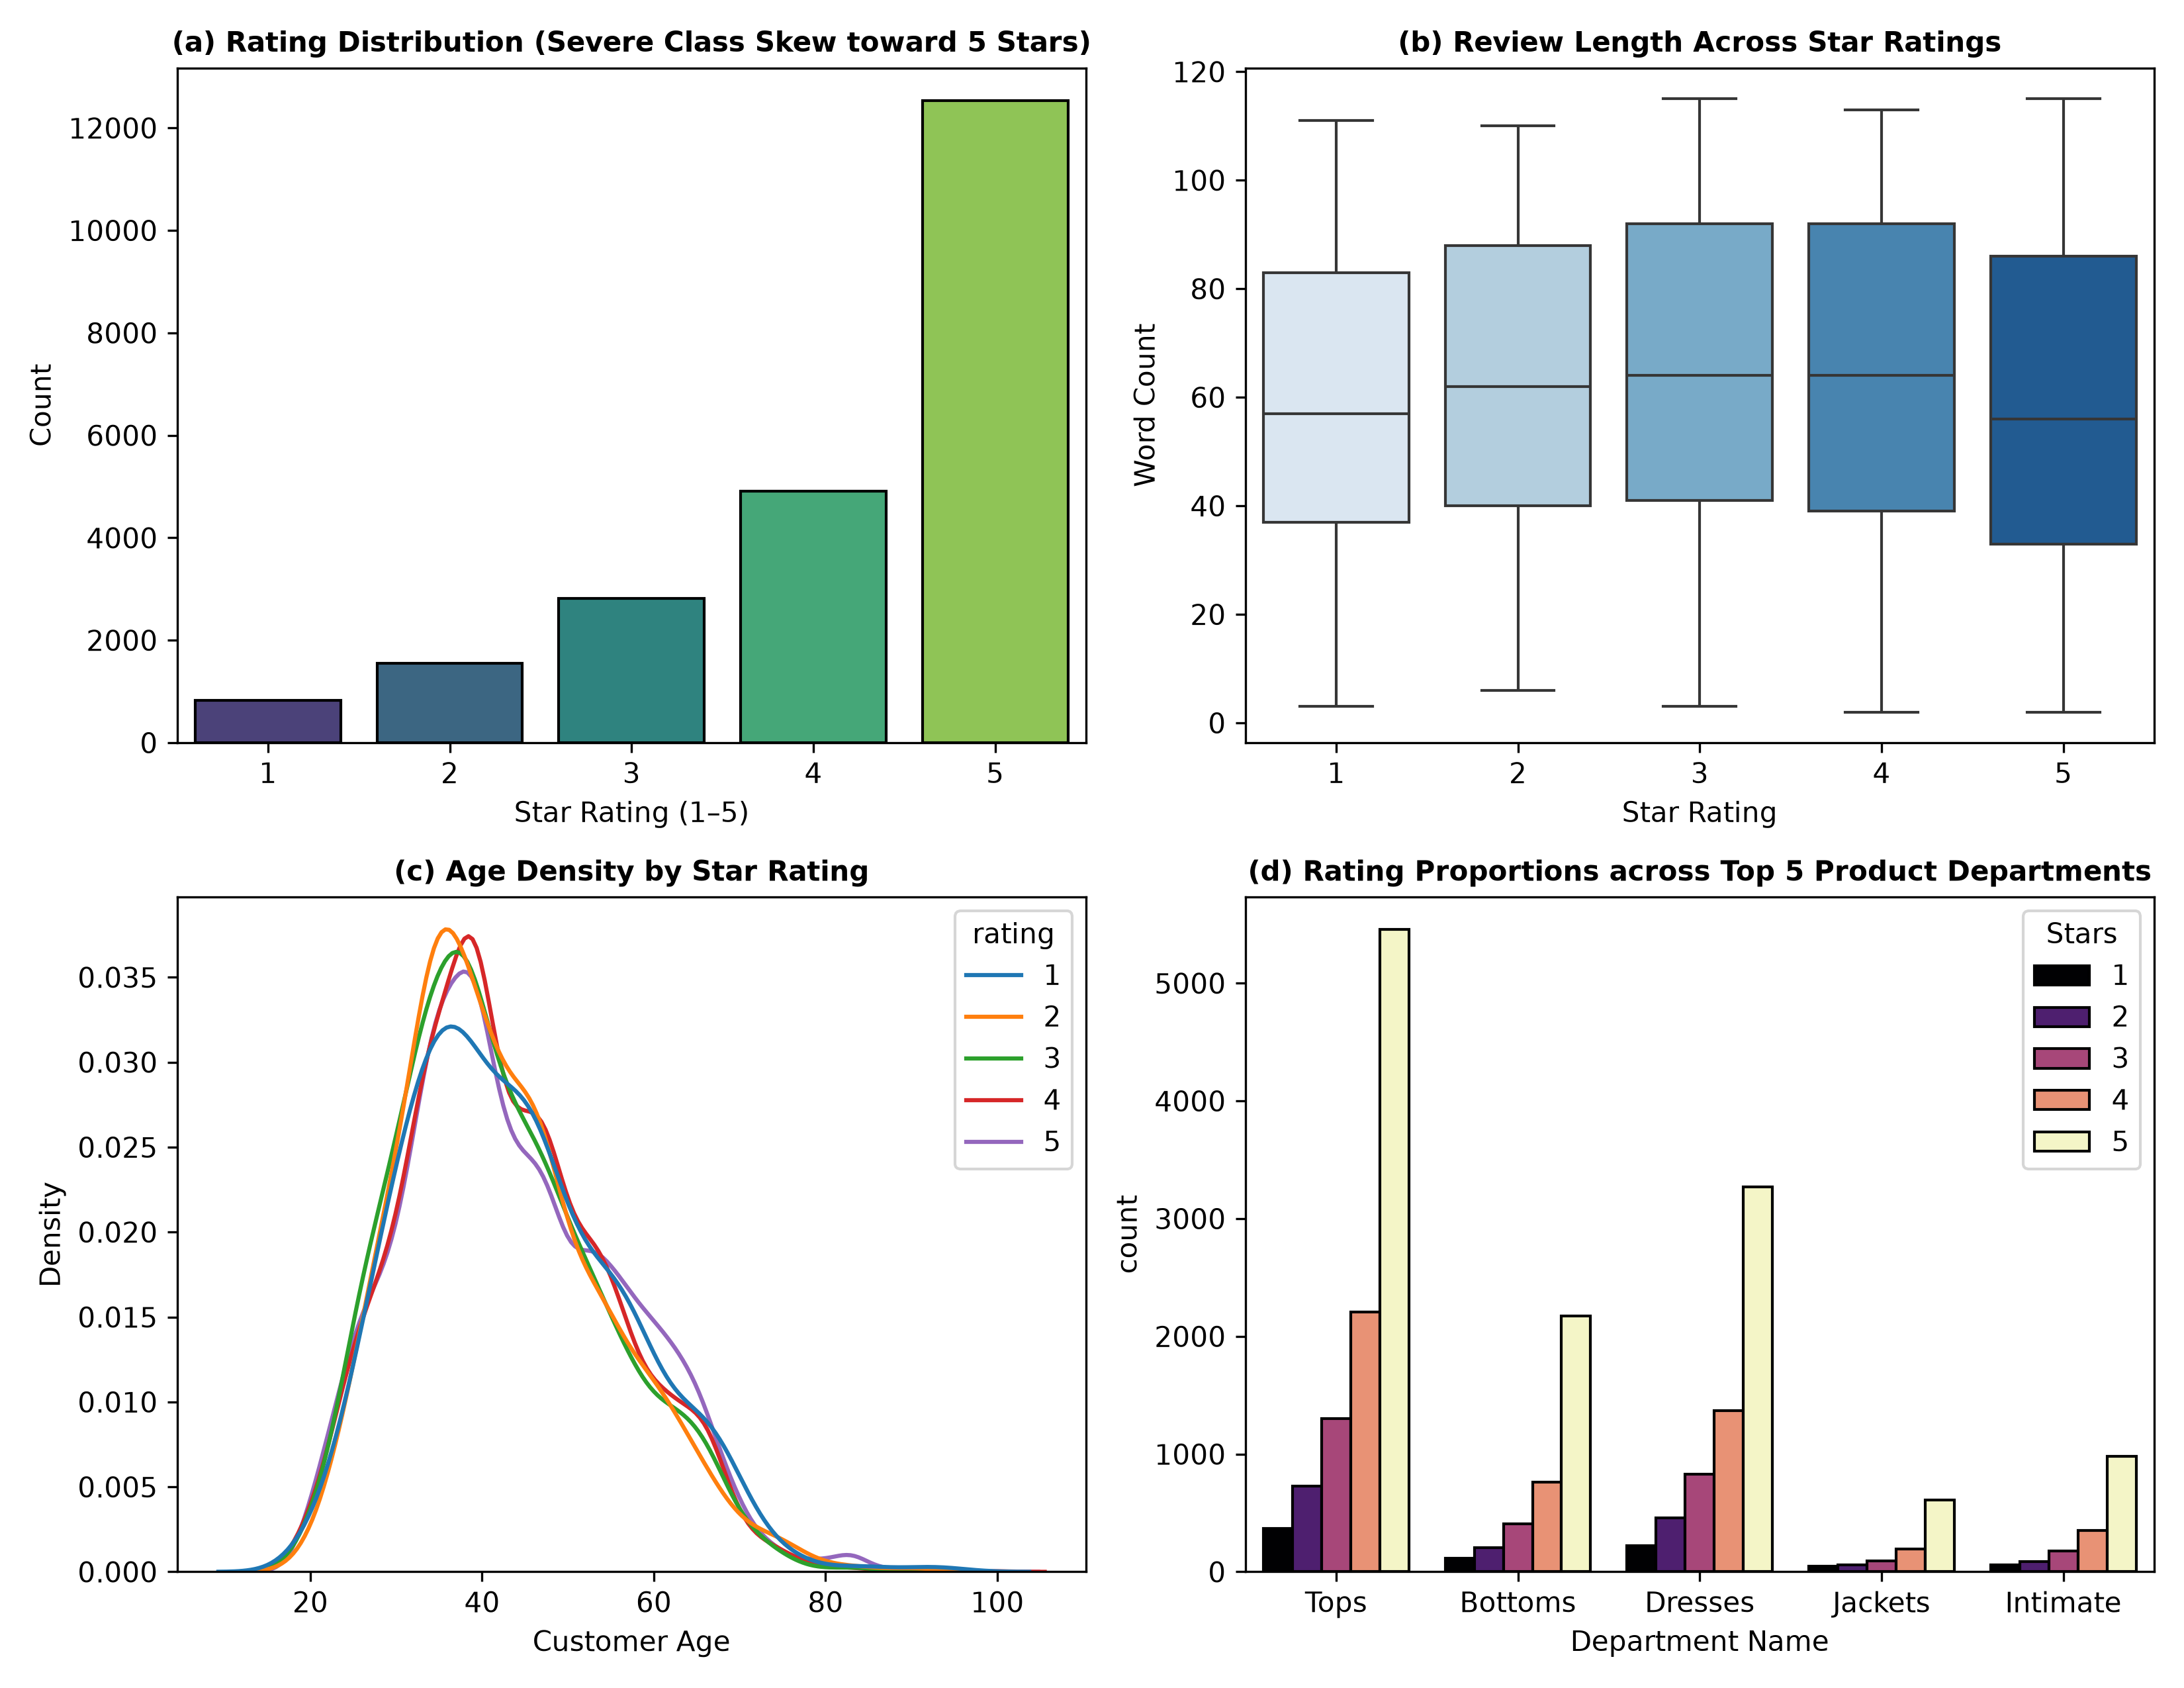
\includegraphics[width=0.48\textwidth]{../../figures/eda_clothing_distributions.png}
\caption{Exploratory distributions: (a) Rating counts showing severe 5-star skew; (b) Review length by rating; (c) Age density; (d) Rating distribution across departments.}
\label{fig:eda_clothing}
\end{figure}

\section{Methodology}
\subsection{Data Partitioning & Preprocessing Pipeline}
The dataset is split into a stratified 70/15/15 train/validation/test partition ($\text{seed}=42$).
We structure three preprocessing pipelines:
\begin{enumerate}
\item \textbf{Structured Features:} Numeric age, $\log(1 + \text{feedback})$, and review length scaled via \texttt{StandardScaler}; division, department, and class encoded via \texttt{OneHotEncoder}.
\item \textbf{Text Features:} TF-IDF vectorizer (uni- and bi-grams, max 5,000 features, English stop words removed).
\item \textbf{Multimodal Fusion:} Concatenation of both pipelines within a single \texttt{ColumnTransformer}.
\end{enumerate}

\subsection{Model Portfolio & Re-Framing}
We evaluate Logistic Regression (unweighted vs. balanced), Linear SVM, and Random Forest. We further train a re-framed 3-class classifier mapping ratings into Negative (1--2), Neutral (3), and Positive (4--5).

\section{Results}
Table~\ref{tab:results} summarizes the 5-class ablation and 3-class results on the held-out test set (3,397 samples). Linear SVM achieved champion 5-class performance (Macro-F1 0.3958, Ordinal MAE 0.5131), while balanced weighting maximized Macro-F1 (0.4335). Re-framing into 3 commercial sentiment tiers boosted accuracy to 81.63\% (Macro-F1 0.5540).

\begin{table}[htbp]
\caption{Ablation study and 3-class re-framing results on test set.}
\label{tab:results}
\centering
\begin{tabular}{lrrrr}
\toprule
\textbf{Model / Modality} & \textbf{Acc} & \textbf{Macro-F1} & \textbf{W-F1} & \textbf{Ord. MAE} \\
\midrule
Structured-Only & 0.5540 & 0.1426 & 0.3950 & 0.8160 \\
Text-Only & \textbf{0.6314} & 0.3830 & 0.5915 & \textbf{0.5004} \\
Combined (Unweighted) & 0.6273 & 0.3756 & 0.5876 & 0.5110 \\
Combined (Balanced) & 0.5890 & \textbf{0.4335} & \textbf{0.6011} & 0.5508 \\
Combined (Linear SVM) & 0.6135 & 0.3958 & 0.5896 & 0.5131 \\
\midrule
3-Class Re-Framed & \textbf{0.8163} & \textbf{0.5540} & \textbf{0.7883} & -- \\
\bottomrule
\end{tabular}
\end{table}

\begin{figure*}[t]
\centering
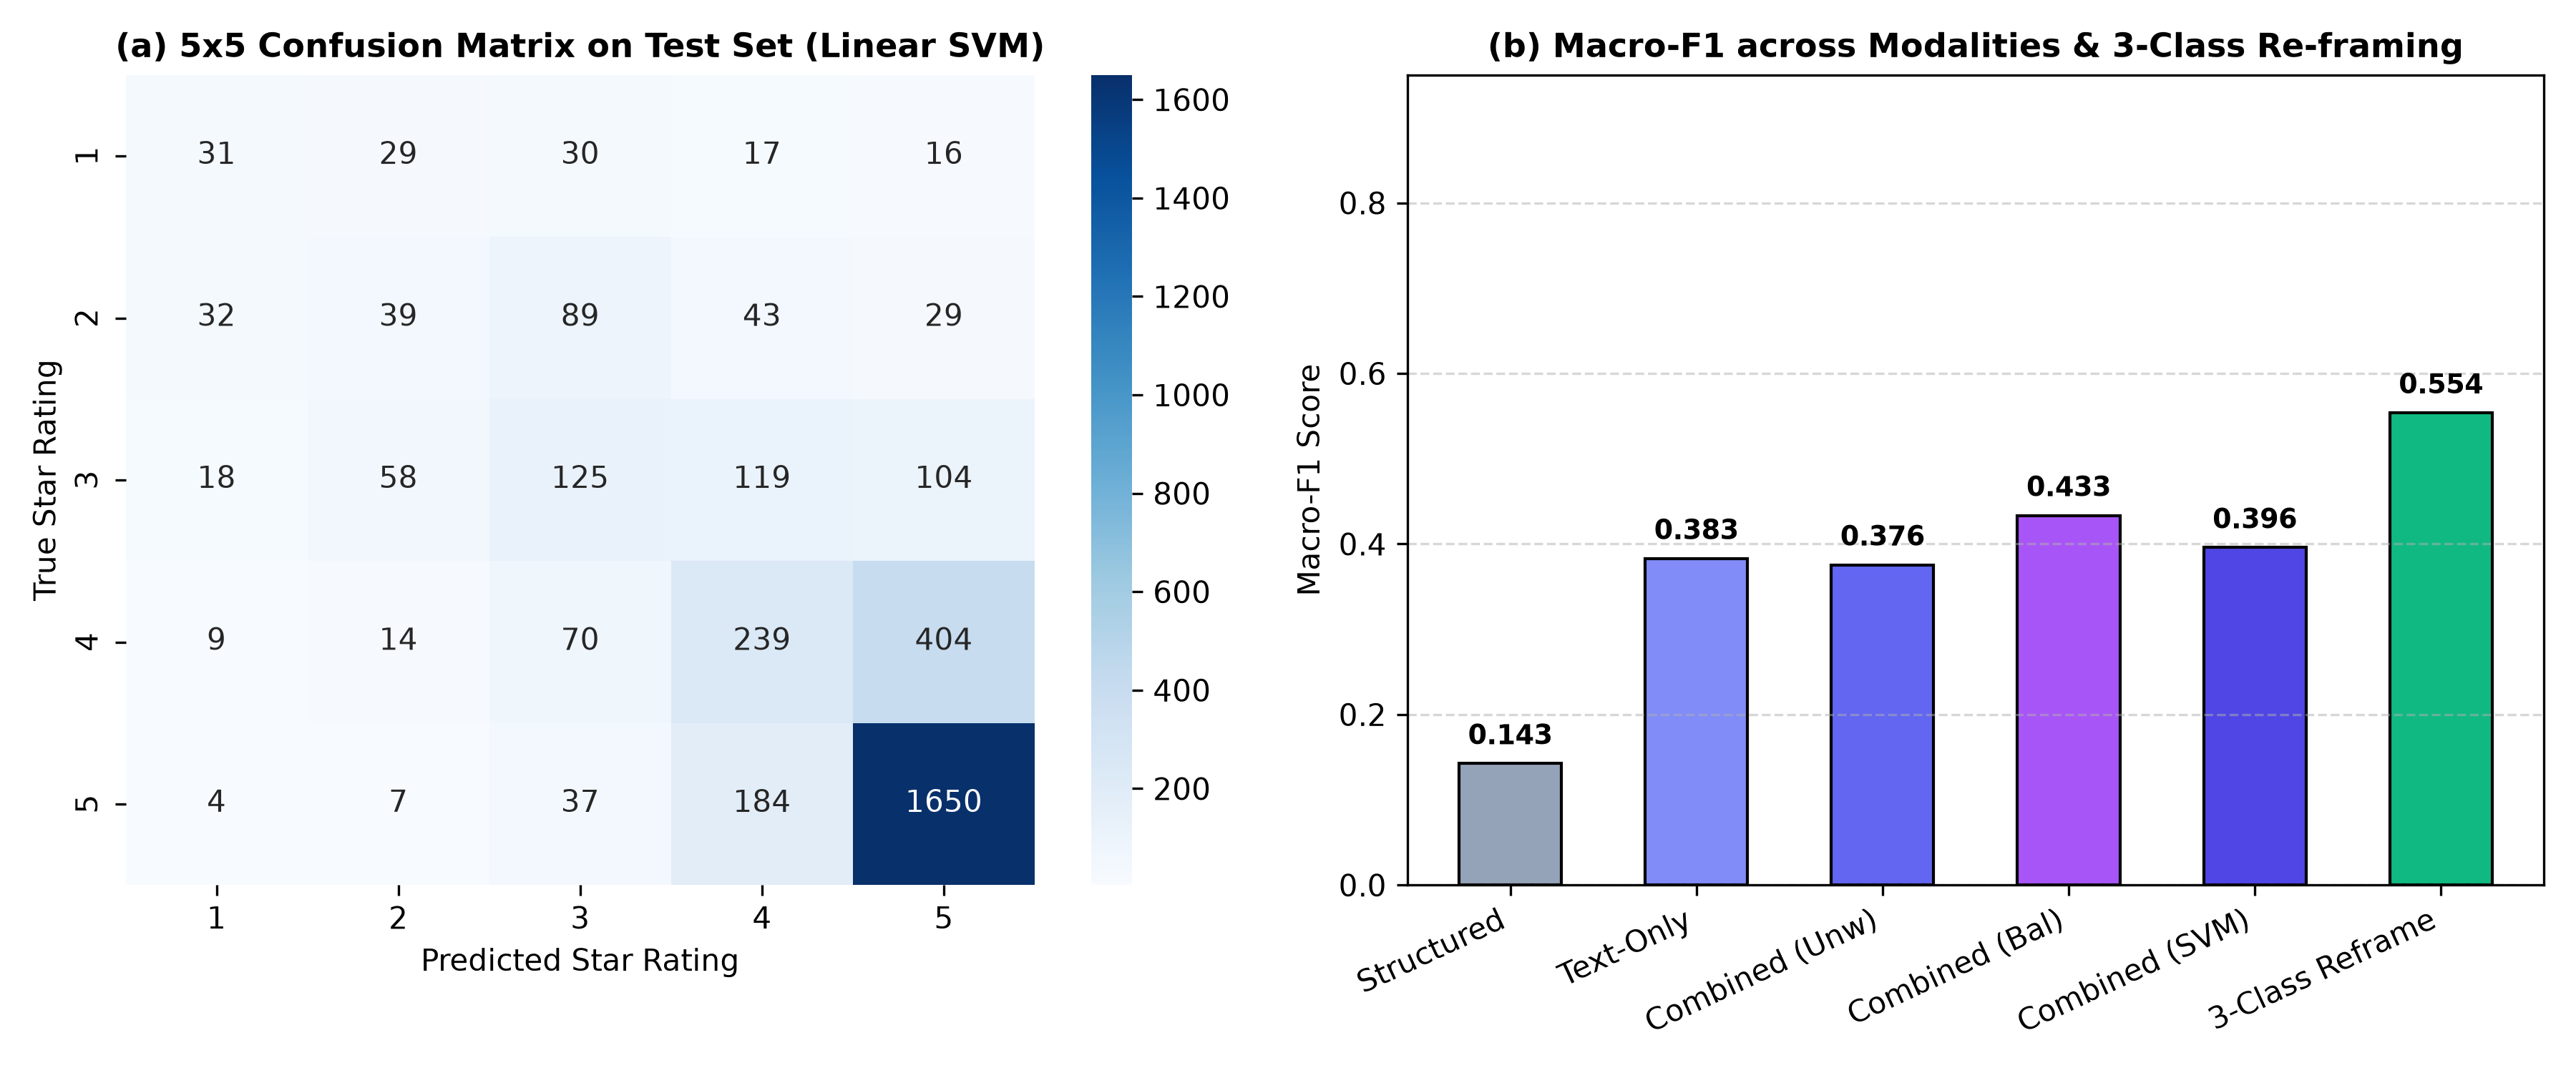
\includegraphics[width=0.98\textwidth]{../../figures/combined_key_result.png}
\caption{Key experimental results: (a) $5 \times 5$ confusion matrix for Linear SVM showing dominant off-by-one confusion between 4 and 5 stars; (b) Macro-F1 across feature modalities and the commercial 3-class re-framing.}
\label{fig:combined_key_result}
\end{figure*}

\section{Discussion & Analysis}
\subsection{Confusion Dynamics: The 4 vs. 5 Star Ambiguity}
The confusion matrix in Fig.~\ref{fig:combined_key_result}(a) indicates that the largest error concentration occurs between 4 stars and 5 stars (over 480 4-star reviews predicted as 5 stars). This stems from \textbf{subjective consumer label noise}: two reviewers expressing identical satisfaction (\textit{``Great fit, soft fabric, love the color''}) often diverge arbitrarily between 4 and 5 stars based on personal grading scales rather than semantic differences. The low Ordinal MAE (0.513) confirms that nearly all errors are off-by-one.

\subsection{Contribution of Structured Metadata}
Structured administrative features alone yield a poor Macro-F1 of only 0.1426 (collapsing to majority-class prediction). Adding metadata to text produces virtually identical accuracy (0.6314 vs. 0.6273), demonstrating that customer review text contains overwhelmingly dominant predictive power.

\subsection{Business Utility of 3-Class Re-Framing}
Fine-grained differentiation between 4 and 5 stars offers minimal utility for e-commerce inventory decisions. Grouping into Negative (1--2), Neutral (3), and Positive (4--5) allows automated triage of customer dissatisfaction, elevating operational classification accuracy to 81.63\% (Macro-F1 0.5540).

\section{Conclusion}
Multimodal text classification successfully predicts consumer clothing review ratings. Excluding \texttt{Recommended IND} was critical to prevent label leakage. Class weighting improved minority Macro-F1, and 3-class reframing maximized operational business value.

\newpage
\section*{AI Use Disclosure Statement}
\begin{itemize}
\item \textbf{AI Tool Utilized:} Google Antigravity Agent (Gemini 2.5 Pro).
\item \textbf{Scope of Assistance:} Scaffolding multimodal ColumnTransformers, ordinal classification metrics, and IEEE two-column report compilation.
\item \textbf{Human Verification:} All models and reframing evaluations were executed locally with fixed random seeds ($\text{seed}=42$); all reported numbers match notebook outputs 1:1.
\end{itemize}

\begin{thebibliography}{00}
\bibitem{nicapotato2018} S. Nicapotato, ``Women's E-Commerce Clothing Reviews,'' \textit{Kaggle Dataset}, 2018.
\bibitem{pedregosa2011} F. Pedregosa \textit{et al.}, ``Scikit-learn: Machine learning in Python,'' \textit{J. Mach. Learn. Res.}, vol. 12, pp. 2825--2830, 2011.
\end{thebibliography}

\end{document}
